\documentclass[../thesis_seyed.tex]{subfiles}
% \graphicspath{{\subfix{../img/}}}
\begin{document}
\chapter{DIFFERENTIAL THETA-BAND SIGNATURES OF THE ANTERIOR CINGULATE AND MOTOR CORTICES DURING SEATED LOCOMOTOR PERTURBATIONS}
\section{Introduction}
\label{sec:introduction}
Perturbing locomotion often produces error-driven adaptation where subjects adjust their locomotor patterns to reduce errors, but these adjustments revert to the unperturbed patterns after the perturbations are removed (i.e. wash-out) \cite{Torres-Oviedo2011-tv} \footnote{This chapter has been published in the IEEE Transactions on Neural Systems and Rehabilitation Engineering, doi:10.1109/TNSRE.2021.3057054}. {When subjects are re-exposed to the same perturbations or exposed to new perturbations, they adapt faster and may also modify unperturbed locomotor patterns} \cite{Leech2018-sr}. {However, these modifications may not transfer across lower limbs according to a split-belt walking study} \cite{Choi2007-pc}. {Despite the wash-out often seen with error-driven adaptation, split-crank cycling and split-belt walking can result in retained post-perturbation modifications if the modifications were not the direct task goals} \cite{Alibiglou2011-sc,Maclellan2014-vk}. For example, after cycling with different crank angles, subjects had perturbation-specific muscle activation patterns which did not wash-out post-perturbation \cite{Alibiglou2011-sc}. These locomotor behaviors indicate that perturbations indeed modify locomotor responses beyond the perturbation period and that tuning perturbation features could modulate locomotor responses. Determining motor and cortical responses to different perturbations during a variety of locomotor tasks, beyond just walking, could greatly improve the understanding of locomotor adaptation processes.

Advancements in brain imaging technologies such as high-density electroencephalography (EEG), functional magnetic resonance imaging, and positron emission tomography have helped researchers identify supra-spinal correlates of locomotion \cite{Gramann2011-yj,Enders2016-id,Hinton2019-gg}. The anterior cingulate cortex theta (3-8 Hz) power increases significantly during double-support in walking and during extension-onset in recumbent stepping \cite{Bulea2015-dv,Kline2016-ci}. These studies suggest that the anterior cingulate activity may be monitoring more demanding locomotion phases. The supplementary motor area (SMA) has similar theta power fluctuations during walking, cycling, and recumbent stepping \cite{Gramann2011-yj,Jaeger2014-ao,Kline2016-ci}. In general, the SMA and the motor cortex exhibit substantial alpha-beta (8-30 Hz) fluctuations during walking, with decreased alpha-beta power indicating active processing in the motor cortex \cite{Nordin2019-gd}.

The anterior cingulate cortex and SMA also both strongly respond to perturbations during walking and standing. Previous studies on split-belt walking, perturbed beam walking, walking over obstacles, and perturbed stepping reported perturbation-elicited activity of anterior cingulate, SMA, or in both areas \cite{Haefeli2011-ym,Bulea2015-dv,Marchal-Crespo2017-fn,Peterson2018-ht,Hinton2019-gg,Nordin2019-ar}. The anterior cingulate cortex (or the equivalent mid-prefrontal cortex in the EEG channel studies) activity is often associated with error monitoring or motor learning, while SMA activity is associated with sensorimotor integration \cite{Ridderinkhof2004-jx,Galea2011-jf,Peterson2018-ht}. If the anterior cingulate cortex has an error monitoring function, we expect that the activity would scale with the error size \cite{Arrighi2016-yb}. If the anterior cingulate has a role in motor learning, we expect the activity would decrease with more perturbation experience. Previous studies on walking over obstacles and perturbed standing did not observe decreased anterior cingulate activity with more experience \cite{Haefeli2011-ym,Mierau2015-fd}. On the other hand, a recent study reported scaling of central midline EEG signals at the Cz electrode with balance performance during a perturbed standing task \cite{Payne2020-hl}. However, all three studies had insufficient spatial resolution to determine confidently whether the electrocortical dynamics were from a single functional cortical area.

The purpose of this study was to determine the electrocortical signatures of motor responses to perturbations during a seated locomotor task.
%  To our knowledge, there are no studies that have investigated locomotor adaptation and their electrocortical correlates during a seated locomotor task.
Adding perturbations during seated locomotor tasks such as recumbent stepping, which likely shares neural control with walking \cite{Stoloff2007-da,Zehr2007-ww} could provide an alternative option for gait rehabilitation since subjects do not need to maintain their balance. Using our motorized recumbent stepper \cite{Huang2009-of}, we applied discrete mechanical perturbations during each stride and also had intermittent no-perturbation "catch" strides. The catch strides could probe whether subjects were updating anticipatory motor control strategies.
%  We used high-density EEG, independent component analysis (ICA), and a source estimation technique to identify activity of cortical sources during this experiment.

We had four hypotheses. The first hypothesis was that perturbations would initially create motor errors and increase anterior cingulate theta power near the perturbation event. As subjects gained more experience with perturbations, motor errors, and anterior cingulate theta power would decrease. The second hypothesis was that motor errors during the no-perturbation catch strides would increase the more subjects expected to encounter perturbations and that anterior cingulate spectral fluctuations would decrease in the later catches. The third hypothesis was that mid-extension perturbations, when the limbs were moving the fastest, would produce more significant errors and anterior cingulate theta power than extension-onset perturbations. We also expected to identify activity of the left and right motor cortices \cite{Jaeger2014-ao,Kline2016-ci} and hypothesized that spectral power fluctuations of the left and right motor cortices in response to the perturbations would be lateralized.

\begin{figure}[!t]
\centerline{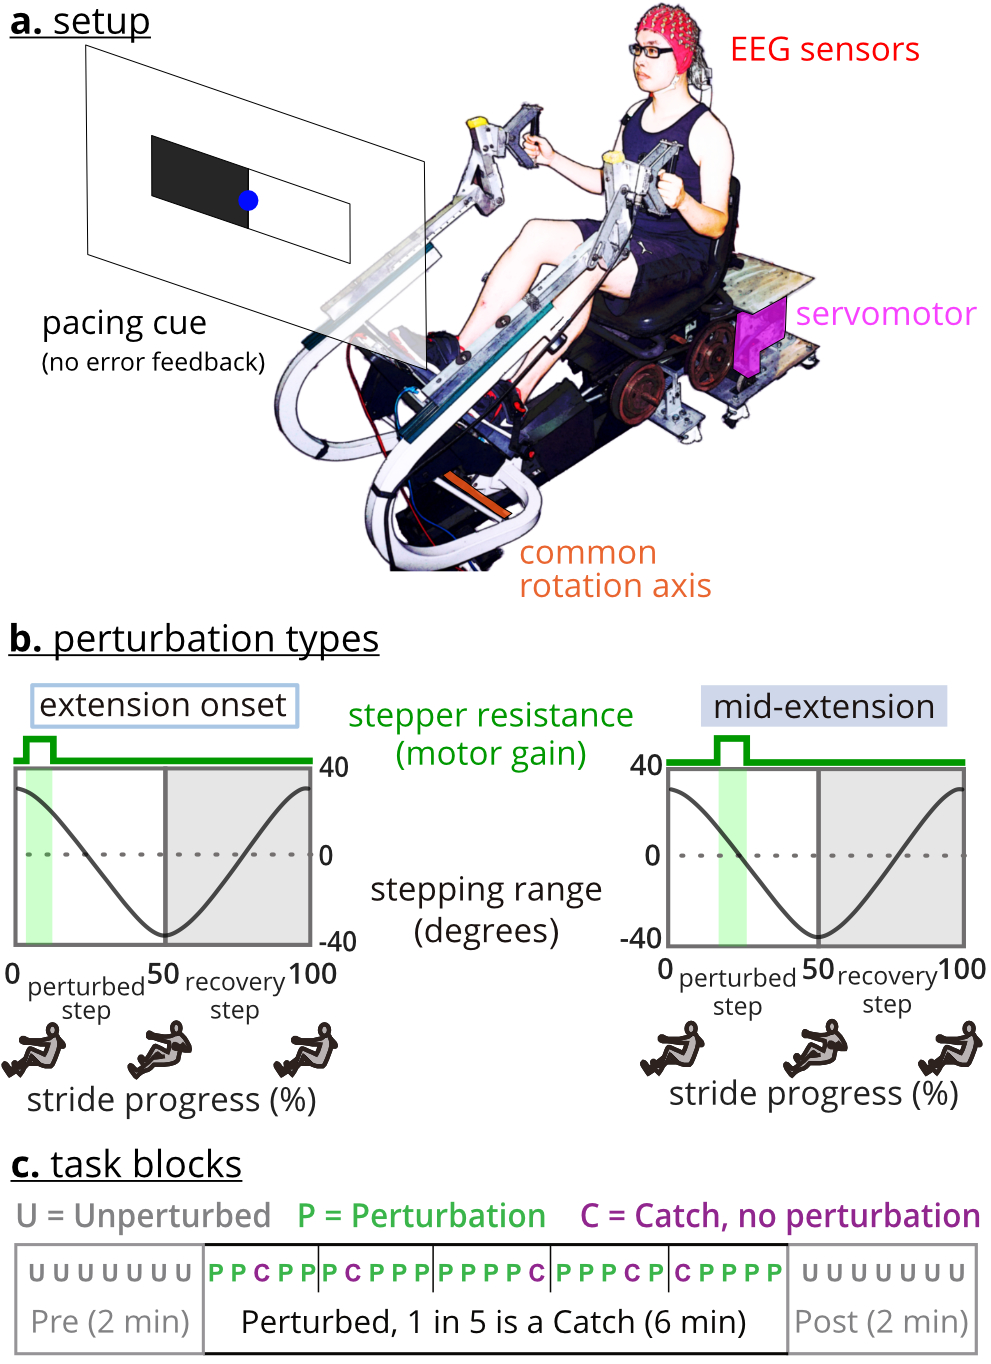
\includegraphics{../img/01_device-protocol_errorMetric.jpg}}
\caption{\textbf{Recumbent stepper and perturbations.} \textbf{a.} The recumbent stepper is a one-degree-of-freedom arm-leg exercise device. \textbf{b.} Perturbations were applied either at the extension-onset or mid-extension of the targeted leg. Perturbations were increased stepping resistance for 200 milliseconds. \textbf{c.} The experiment included four tasks. Each task had three ordered blocks, pre, perturbed stepping, and post. The perturbed stepping block also included random no-perturbation catch strides.}
\label{fig:fig1}
\end{figure}

\section{Methods}
\label{sec:methods}
Subjects (n=17, 11 females, age 25 ± 4.9 years) performed perturbed arm-leg stepping on a one degree-of-freedom recumbent stepper {(TRS 4000; NuStep, Inc., Ann Arbor, MI)} integrated with a servomotor {(Kollmorgen, Radford, VA), described in }\cite{Huang2009-of} (Figure \ref{fig:fig1}a). The mechanically coupled left handle and right pedal move together out of phase with the mechanically coupled right handle and left pedal. As such, subjects could use any combination of their arms and legs to drive the stepper.

\subsection{Experiment procedure and motor errors}
The Institutional Review Board of the University of Central Florida approved the protocol and consent form, and the study was conducted per the principles stated in the Declaration of Helsinki. All subjects gave their written informed consent before starting the experiment. Subjects were all right-handed, based on the hand they would use to pick an object from the floor. Subjects self-reported no prior neurological or musculoskeletal problems in the past two years before the data collection date.

We recorded EEG using a 128-electrode EEG system (ActiveTwo, BioSemi B.V., Amsterdam, the Netherlands). After placing the EEG cap on the subject’s head according to the BioSemi guidelines, we digitized the electrodes and fiducial locations using an infrared 3D scanner (Structure Sensor, Occipital Inc., Boulder, CO). We ensured that the resistance between the scalp and each electrode was <20 Ohms, indicating good contact between the electrodes and the scalp. We restrained cable movement using a cable holder behind the subject’s head and instructed subjects to keep their head steady to reduce EEG cable sway artifacts \cite{Symeonidou2018-ge}. We strapped subjects' feet to the pedals after they sat on the stepper seat. We also adjusted the handles to ensure that subjects were comfortable using the handles to drive the stepper.

The stepper’s servomotor perturbed the stepping motion with brief 200 ms increases in resistance at either the onset or middle of extension of the target (left or right) leg during the stepping stride (Figure \ref{fig:fig1}b). The increased resistance magnitude during a perturbation required 3x the torque to maintain the stepping pace of 60 steps per minute. In total, there were four perturbation types (left/right leg * mid-extension/extension onset). A {pacing cue} equal to 60 steps per minute (=30 strides per minute) was provided {on a visual display to help subjects} maintain similar stepping speeds during and across tasks. 

EEG was recorded at 512 Hz using the BioSemi software program{, and the stepping kinematics were recorded using the servomotor's encoder at 100 Hz in the stepper program. When the stepper program began and ended,} a trigger signal was sent to start and stop the EEG recording to synchronize the data.

\begin{figure}[!t]
\centerline{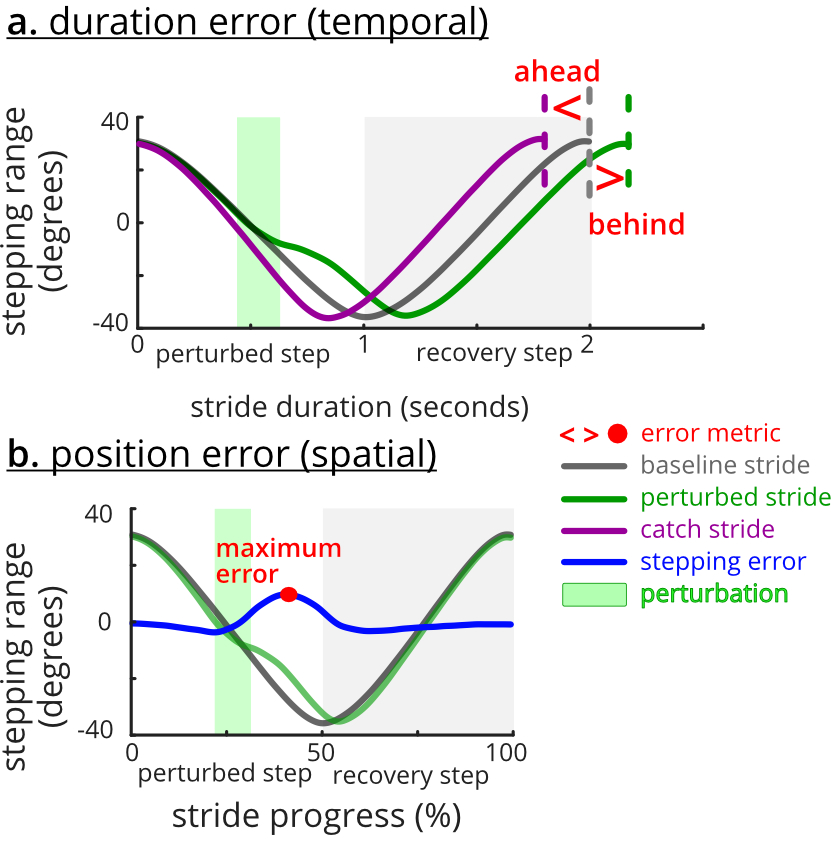
\includegraphics{../img/02_error_metrics.jpg}}
\caption{\textbf{Motor error metrics.} Subjects were instructed to match the pace and step smoothly. \textbf{a.} Stepping duration (i.e., temporal) error is the difference between stride duration and the two-second pacing cue. \textbf{b.} Stepping position (i.e., spatial) error is the maximum difference between the time-normalized stepping profile and the averaged \textit{pre} profile.}
\label{fig:fig2}
\end{figure}
\subsubsection{Data collection}
The data collection began with two minutes of quiet sitting, during which the  pacing cues were shown as EEG was recorded. After completing this quiet sitting portion, subjects completed four 10-minute perturbed stepping \textit{\underline{tasks}} in a pseudo-randomized order. Each task only included one perturbation type. For each task, there were three ordered \textit{\underline{blocks}}: 1) \textbf{pre}: two minutes of unperturbed stepping, 2)  \textbf{perturbed stepping}: six minutes of a single perturbation timing, and 3)  \textbf{post}: two minutes of unperturbed stepping (Figure \ref{fig:fig1}c). There were no pauses between blocks. In addition to perturbed strides, the perturbed stepping block included random one-in-five “catch” strides where no perturbation was applied. In this paper, we use pre and pre-perturbation and post and post-perturbation interchangeably. There was two minutes of quiet sitting at the end of the data collection.

Before starting each task, we instructed subjects to \textbf{A)} step smoothly as if they were walking, \textbf{B)} use both their arms and legs to drive the stepping motion, and \textbf{C)} follow the  pacing cues that were projected in front of them (Figure \ref{fig:fig1}a). We did not instruct subjects on how to follow the pacing cues as there are several options, such as having a leg be at full extension when the rectangle on the same side as the leg was black. Subjects also received no explicit feedback on whether they were stepping faster or slower than the pacing cue. Subjects were given at least two minutes of practice with the  pacing cues before starting the data collection.

\subsubsection{Stride events}
After importing stepping data into MATLAB (R2018b, MathWorks Inc, Natick, MA), we separated each task into blocks and strides. We defined the strides as the time from one extension-onset of the perturbed leg to the next extension-onset of the perturbed leg. We excluded any incomplete strides. For each stride, we identified the following \textit{\underline{events}}: perturbed-step extension onset, perturbation (start time), recovery-step extension onset, and the end of the stride. We artificially added perturbation events to the unperturbed strides (i.e., pre, post, and catch strides), equal to the average latency of the perturbation events.

\subsubsection{Motor errors}
We quantified a temporal (pacing) error and a spatial (stepping) error, from the stepping kinematics (Figure \ref{fig:fig2}). In our tasks, subjects should have completed a stride in two seconds based on the 60 steps-per-minute pacing cues. We defined temporal error as the stepping duration error, which was the difference between each stride duration and the two seconds (Figure \ref{fig:fig2}a). Since we instructed subjects to step smoothly, we expected the stepping profiles to be smooth and rhythmic during the pre-perturbation block. We defined spatial error as a stepping position error, which was the maximum difference between the time-normalized stepper position profile during each stride and the averaged pre-perturbation stepping profile (Figure \ref{fig:fig2}b). We used the servomotor encoder data to quantify the angular stepping position around the stepper's common rotating axis (Figure \ref{fig:fig1}a).

\subsection{EEG processing}
EEG data were analyzed in MATLAB (R2018b, MathWorks Inc, Natick, MA) using a customized pipeline based on EEGLAB (version 2019.0) functions \cite{Delorme2004-yy} (Figure \ref{fig:fig3}). We used a high-pass filter at 1 Hz and a 60 Hz line-noise filter (CleanLine) to minimally clean the raw data \cite{Mullen2012-rh,Winkler2015-br}. We imported stride events from the synchronized stepping data and concatenated data from all tasks into a single file. We then used a template correlation rejection method to identify and exclude channels with large cyclic artifacts \cite{Oliveira2017-pk}.

\begin{figure*}[!ht]
\centerline{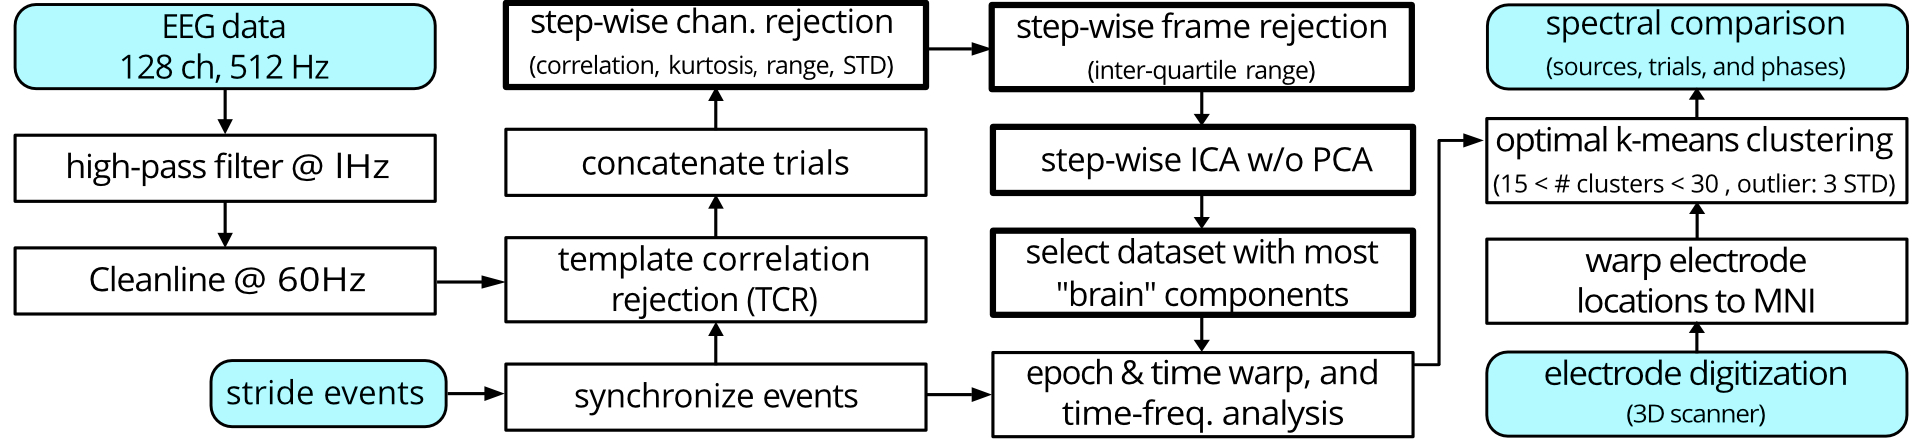
\includegraphics{../img/03_EEG workflow.jpg}}
\caption{\textbf{EEG post-processing workflow with a novel step-wise algorithmic parameter sweeping noise rejection process.} Shaded blocks indicate inputs or outputs. Thick lined blocks highlight the novel step-wise rejection approach.}
\label{fig:fig3}
\end{figure*}

We developed and used a novel step-wise channel and frame rejection algorithm to reject channels and data frames that still contained considerable noise (Figure \ref{fig:fig3}). We removed the researcher's need to set single thresholds for the channel and frame rejection steps. Instead, the step-wise algorithm identified a suite of thresholds, from lenient to conservative, that created 32 separate datasets with different rejection levels for each participant (8 steps for channel rejection * 4 steps for data-frame rejection = 32 datasets). Channel rejection metrics were the signal range, standard deviation, kurtosis, and correlation to the other channels. Frame rejection involved finding periods of the EEG data with a significantly higher signal variability than the overall median of signal variability. While the number of the rejected channels and frames varied for each participant and increment, we set the rejection thresholds such that the most conservative increment always retained > 85 channels and > 80\% of data.

We used independent component analysis (ICA), the dipolar source estimation technique (DIPFIT), and a multi-variate source classifier (ICLabel) on each step-wise dataset to identify and locate the sources that contributed to the EEG signals. We specifically used the adaptive mixture independent component analysis (AMICA) to separate the EEG into temporally independent components \cite{Palmer2008-jx}. To select the best increment from the 32 step-wise datasets, we first estimated the source locations for each dataset's independent components using EEGLAB’s DIPFIT version 3.0. We then excluded any source located outside the brain or with the residual variance > 15\%. We then used EEGLAB’s ICLabel toolbox to classify the source types as “brain” or “non-brain” \cite{Pion-Tonachini2017-ez} and selected the step-wise dataset with the topmost “brain” sources as the representative dataset for each subject. We visually checked the results of the ICLabel for the selected dataset to confirm the classification of the sources as “brain” (or “non-brain”).

We then clustered the sources across all subjects based on the source location, power spectrum, and scalp map. We divided the power spectrum and scalp map into ten bins. The binned power spectrum was from 3 to 25 Hz. The Laplacian of the scalp map was used for clustering \cite{Hjorth1975-ea}. We developed and used a novel optimal k-means approach to determine the number of clusters from a range of possible numbers of clusters provided to the algorithm (here, from 15 to 30 clusters). The optimal k-means approach uses MATLAB’s “evalcluster” function to find the specific number of clusters that maximize the similarity of the sources within each cluster. We kept and analyzed only the clusters that contained components from more than 70\% of the subjects. If a subject had multiple sources in a cluster, we only kept the source with the largest channel data variance. We identified Brodmann Areas and cortical cortices of the sources and cluster centroids using Talairach coordinates and \href{http://talairach.org/}{talairach.org} \cite{Lancaster2000-aj,Shirazi2019-im}.

We computed the time-frequency spectral power of each source in the cluster across the stride epochs, known as event-related spectral perturbations (ERSP) \cite{Makeig1993-jx}. For hypotheses 1, 2, and 4, each epoch was a stride, and for hypothesis 3, each epoch was –400 ms to +400 ms of the perturbation event. We padded the epochs by 700 ms to avoid possible edge effects. Next, we baseline-normalized the spectral power based on the pre-perturbation block's average spectral power and computed the ensembled average ERSPs across subjects. We determined the significant event-related synchronization and event-related desynchronization across the ERSPs using EEGLAB’s bootstrapping method with alpha set at 0.05 \cite{Pfurtscheller1999-oi}. ERSP images only show significant spectral fluctuations.

\begin{figure*}[!ht]
\centerline{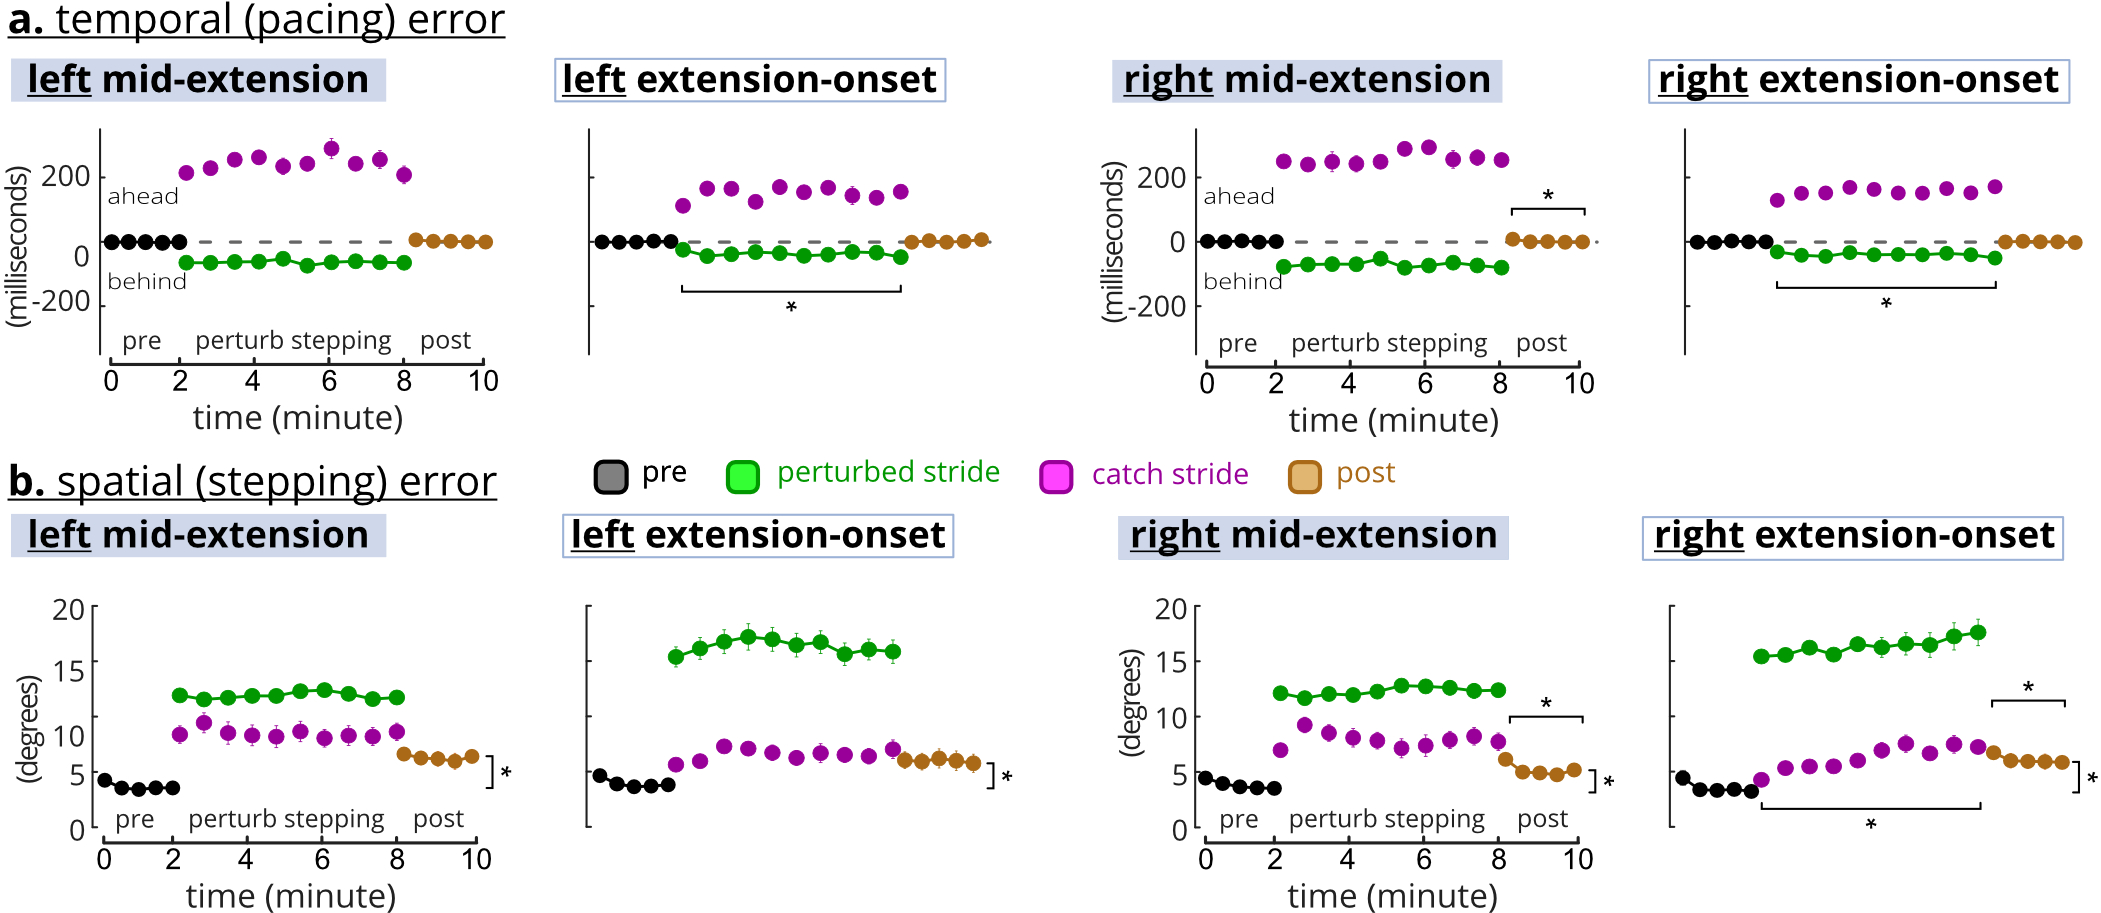
\includegraphics{../img/04_error-result-tnsreR1.jpg}}
\caption{\textbf{Temporal and spatial errors during perturbed stepping.} The \textit{perturbed-stepping} block include both perturbed strides (green) and one-in-five random catch strides (purple). {For \textit{perturbed-stepping}, the 10 circles are the averages of 10\% batches. For \textit{pre} and \textit{post}, the 5 circles are the averages of 20\% batches. * indicates significant post-hoc LSD tests} \textbf{a.} Temporal errors were different between perturbed and catch strides (\td50 ms vs \td200 ms) and returned to the \textit{pre} levels during the \textit{post} block. \textbf{b.} Spatial error was greater for the perturbed strides than catch strides, and did not return to \textit{pre} levels during \textit{post}.}
\label{fig:fig4}
\end{figure*}

\subsection{Statistical analysis}
\subsubsection{Identification of motor responses}
{We tested the temporal and spatial errors to determine the error behavior. For each subject, we divided their strides into 20\% batches in the pre and post blocks and 10\% batches in the perturbed-stepping block} \cite{Van_Leeuwen2019-zb}{. We compared the average of the first and last batches of perturbed strides, catch strides, and post-perturbations strides, as well as the last batch of pre-perturbation strides using repeated-measure analysis of variance (rANOVA) for each error and task. If the rANOVA was significant, we performed a priori Fisher's Least Significant Difference (LSD) tests for the following pairs: 1) late pre vs. late post (for sustained post modifications and wash-out), 2) early vs. late post (for wash-out), 3) early vs. late catch (for adaptation), and 4) early vs. late perturbed (for adaptation). The significance level for all statistical tests was 0.05.}  
\subsubsection{Tests for hypotheses 1 and 2: adaptation of motor and cortical responses}
We compared motor errors and electrocortical dynamics between the early (first 33\% of the strides) and late (last 33\% of the strides) in the perturbed stepping block. {Here, we used 33\% of the strides as early or late to retain at least 10 strides per subject (total perturbed strides$\approx$140-150, total catch strides$\approx$30-40) for EEG group-level analyses} \cite{Makeig1993-jx,Pfurtscheller1999-oi}. We tested motor errors for the perturbed and catch strides separately and used rANOVA with three factors: 1) \textit{adaptation} with two levels: early and late, 2) \textit{task side} with two levels: left and right, and 3) \textit{perturbation timing} also with two levels: mid-extension and extension-onset. We performed post-hoc Student paired t-tests only if the adaptation had a significant main effect because adaptation was the only factor pertinent to our first two hypotheses. To compare the electrocortical responses between early and late perturbed strides and early and late catch strides, we computed the spectral fluctuations and averaged the spectral powers to derive the theta-band (3-8 Hz) ERSP waveform \cite{Pfurtscheller1999-oi,Wagner2016-nx}. We compared the early and late theta-band average ERSP waveforms using bootstrapped paired t-tests {and false discovery rate corrections for multiple comparisons} with EEGLAB’s “statcond” and “fdr” functions. We also determined meaningful spectral-power increases or decreases of the theta-band by determining when the power confidence interval was greater or less than zero. We excluded other frequency bands because preliminary analyses showed the main spectral fluctuations were limited to theta. The significance level for all statistical tests was 0.05.

\subsubsection{Tests for hypothesis 3: effect of perturbation timing}
We included all perturbed strides to quantify possible motor and electrocortical differences between perturbation timings, i.e., mid-extension and extension onset. For each motor error, we used rANOVA with two factors: 1) \textit{perturbation timing} with two levels: mid-extension and extension-onset, and 2) \textit{task side} also with two levels: left and right. We only performed a post-hoc Student paired t-test between the same side tasks if there was a significant perturbation timing effect. We compared the ERSPs centered around the perturbation event for left-side tasks (i.e., left mid-extension and left extension-onset) and right-side tasks separately. Similar to the tests for hypotheses 1 and 2, we used bootstrapped paired t-tests {with corrections for multiple comparisons} to compare the theta-band average ERSP between the tasks and determined meaningful spectral-power increases or decreases when the power confidence interval cleared zero. All statistical tests had 0.05 significance level.

\subsubsection{Tests for hypothesis 4, motor cortex lateralization}
We compared spectral fluctuations of the cortical clusters during the left and right-side tasks to investigate contralateral and specialized lateralization of the motor cortex. Hemispheric activity that corresponds to contralateral limb movements is contralateral lateralization whereas hemispheric activity that corresponds with ipsilateral limb movements is specialized lateralization \cite{Mutha2014-ea}. All perturbed and catch strides were included in this analysis. 

\section{Results}
\label{sec:methods}
\subsection{Motor error responses and cortical clusters}
{Temporal (pacing) and spatial (stepping) errors did not decrease with more exposure to perturbations, and spatial errors did not wash-out (Figure \ref{fig:fig4}). Perturbed-stride temporal errors were \td50 ms but catch-stride temporal errors were \td200 ms (Figure \ref{fig:fig3}a). The rANOVAs indicated significant temporal error differences in each task} (F's\tsu{(6,96)}>40, p's<0.0005). {Post-hoc LSD showed a slight temporal error increase during left and right extension-onset perturbed strides and a temporal error decrease during right extension-onset strides post-perturbation. Spatial errors of perturbed strides were steady, \td12\textdegree{} for mid-extension and \td16\textdegree{} for the extension-onset (Figure \ref{fig:fig3}b). During the mid-extension tasks, catch-stride spatial errors seemed a continuation of pre-perturbation errors at \td5\textdegree{} but trended to \td10\textdegree{} by the end of the catch strides. rANOVAs were significant for the spatial errors across all tasks} (F's\tsu{(6,96)}>29, p's<0.0005).{ Spatial errors did not wash-out (i.e., return to pre) during post-perturbation (post-hoc LSD p's<0.05). However, post-perturbation spatial errors in the right-side tasks decreased from the first to last batch (LSD p's<0.05).}

The optimal k-means identified five cortical clusters (Figure \ref{fig:fig5}). We focused on three clusters located at the anterior cingulate cortex (14 subjects), left SMA (13 subjects), and right SMA (13 subjects). Cluster locations were assigned to the nearest Brodmann areas based on the Talairach coordinates of the cluster centroid \cite{Shirazi2019-im}. As the SMA and premotor cortex share Brodmann area 6, we further confirmed the SMA cluster locations from a previous fMRI and PET meta-analysis \cite{Mayka2006-ye}. The left and right SMA were determined based on the cluster’s centroid location and the individual source locations.
% Ten out of the thirteen left SMA and eleven out of thirteen right SMA sources were on the left or right hemispheres.

\begin{figure*}[!ht]
\centerline{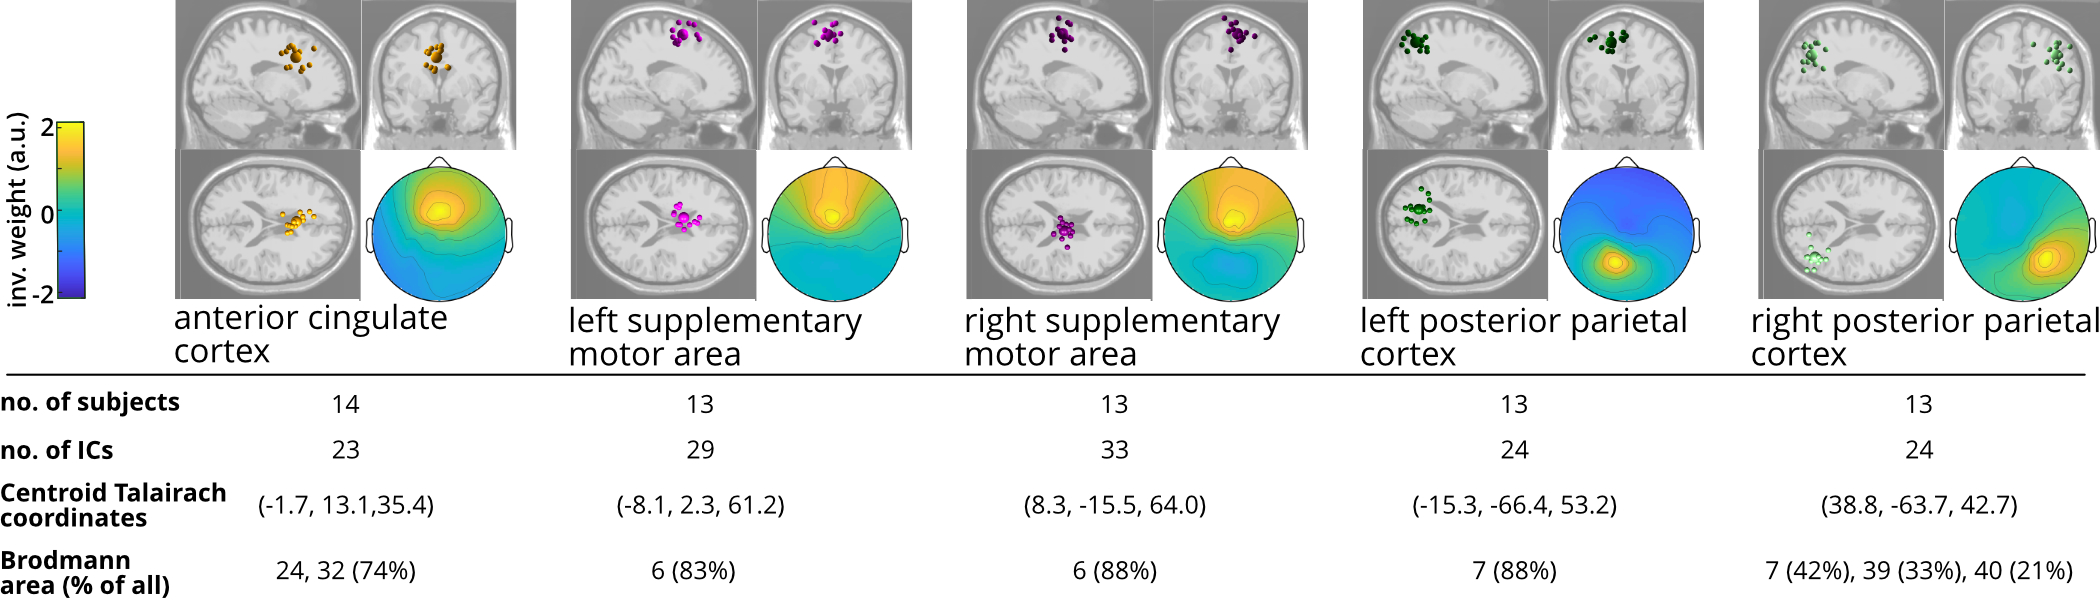
\includegraphics{../img/05_dipole locations_70p.jpg}}
\caption{\textbf{Locations of the electrocortical clusters.} Clusters with sources from > 70\% of the subjects are shown. Only one source per subject was selected for each cluster during analysis. "\% of all" indicates the percentage of all components in the Brodmann Area. a.u.: arbitrary unit}
\label{fig:fig5}
\end{figure*}

\subsection{Anterior cingulate theta-band adaptation occurred without motor error adaptation in perturbed strides}
Motor errors of the perturbed strides did not decrease from early to late, but anterior cingulate theta-band spectral power decreased in the right-side tasks (Figure \ref{fig:fig6}a-c). Neither adaptation nor task side had a significant effect on the perturbed strides (rANOVA, temporal adaptation: F\tsu{(1,16)}=0.74, p=0.789, temporal side: F\tsu{(1,16)}=0.74, p=0.789, spatial adaptation: F\tsu{(1,16)}=2.98, p=0.104, spatial side: F\tsu{(1,16)}=0.71, p=0.413). Mid-extension perturbed strides had significantly greater average temporal errors (71 vs 39 ms) but smaller spatial errors (12\textdegree{} vs 16\textdegree{}) than the extension-onset {perturbed} strides (rANOVA, temporal: F\tsu{(1,16)}=461, p<0.0005, spatial: F\tsu{(1,16)}=30.6, p<0.0005). Perturbations elicited anterior cingulate theta synchronization during all tasks (Figure \ref{fig:fig6}b). Theta spectral power decreased from early to late for right-side perturbed strides. The left-side perturbed strides, however, had similar and sometimes stronger theta synchronization during late strides than the early strides. The anterior cingulate cortex also showed theta desynchronization in the recovery steps (i.e., the unperturbed steps after perturbed steps), specifically for the early right-side and late left-side perturbations. The theta-band average ERSP bootstrap t-tests revealed that spectral power {had a decreasing trend from early to late for the} {right-side tasks, which was significant for right mid-extension perturbations} (Figure \ref{fig:fig6}c). In the left-side perturbed strides, late synchronizations during the recovery steps were statistically different from the non-significant spectral fluctuations during early recovery steps.

\begin{figure}[H]
    \centerline{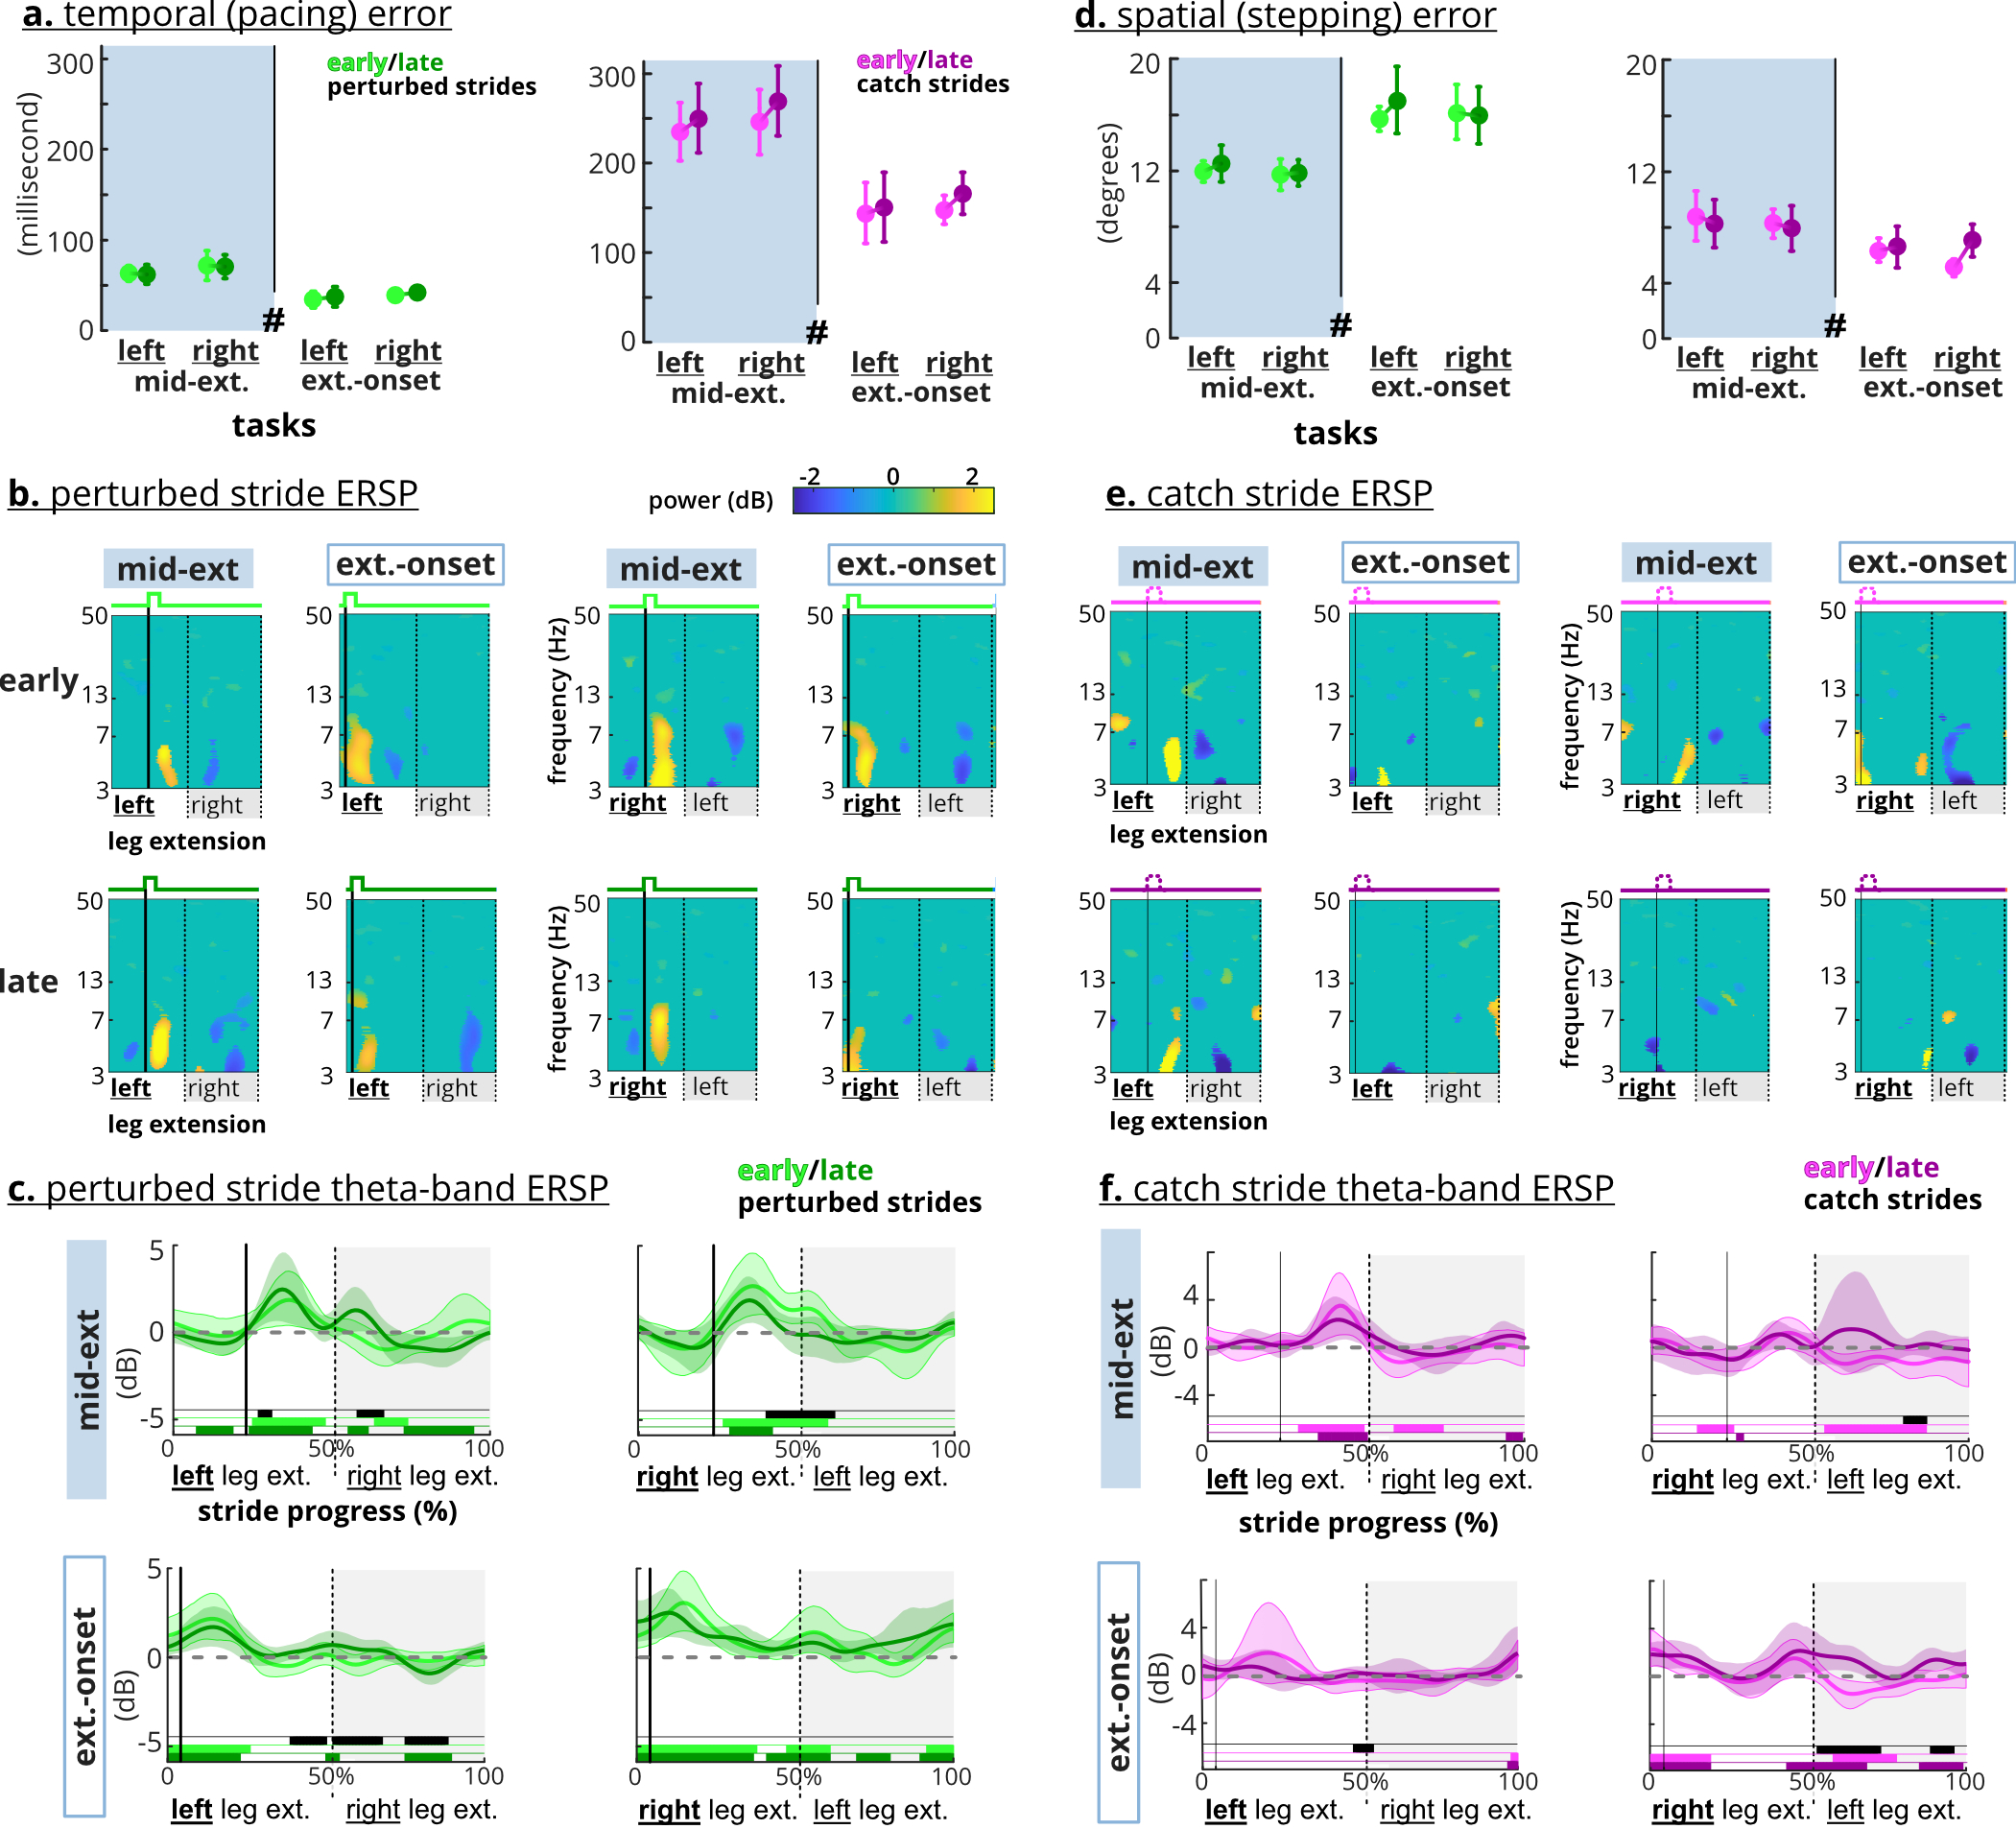
\includegraphics[width=\linewidth]{../img/hyp1and2-fdr.jpg}}
    \caption{\textbf{Motor errors and anterior cingulate ERSP} \textbf{a.} and \textbf{d.} Adaptation (early vs. late) was not a significant factor for motor errors. \# indicates perturbation timing was a significant factor. Error bars indicate confidence interval (CI) \textbf{b.} Perturbations (i.e., the strong solid lines) elicited theta synchronization in anterior cingulate cortex. Right-side perturbations elicited weaker synchronization during the late perturbed strides. \textbf{c.} Average theta-band ERSP waveform shows increased power after the perturbations across the tasks. Late perturbations elicited less theta-band average power only on the right-side tasks. \textbf{e}. Early catches (narrow solid lines) elicited a theta synchronization in the anterior cingulate cortex. \textbf{f.} Average theta-band ERSP waveform shows late right extension-onset catch strides elicited significantly higher spectral power than the early catch. Shaded areas indicate CI. Black bars indicate significant difference between early and late. Colored bars indicate CI does not overlap with zero.}
    \label{fig:fig6}
    \end{figure}

\subsection{Anterior cingulate theta-band adaptation occurred without motor error adaptation in catch strides}
Motor errors did not increase from early to late catch strides, but early catch strides still elicited theta synchronization in the anterior cingulate cortex (Figure \ref{fig:fig6}d-f). Similar to the perturbed strides, neither adaptation nor task side had a significant effect on the temporal or spatial motor errors (rANOVA, temporal-adaptation: F\tsu{(1,16)}=3.76, p=0.070, temporal-side: F\tsu{(1,16)}=1.65, p=0.217, spatial-adaptation: F\tsu{(1,16)}=1.43, p=0.25, spatial-side: F\tsu{(1,16)}=0.70, p=0.415). Mid-extension catch strides had significantly greater average temporal (250 vs 153 ms) and spatial errors (8\textdegree{} vs 6\textdegree{}) than the extension-onset catch strides (rANOVA, temporal: F\tsu{(1,16)}=31.9, p<0.0005, spatial: F\tsu{(1,16)}=24.4, p<0.0005). Early catch steps elicited anterior cingulate theta synchronization (Figure \ref{fig:fig6}e). This synchronization occurred before completion of the catch-step extension for the mid-extension tasks but was near the start of the catch step for just the right extension-onset catch strides. The left mid-extension and right extension-onset elicited theta desynchronization in the recovery steps (Figure \ref{fig:fig6}e-f). For right extension-onset, the recovery steps of the late catch strides elicited significantly greater spectral power than the early catch strides.

\begin{figure}[!h]
\centerline{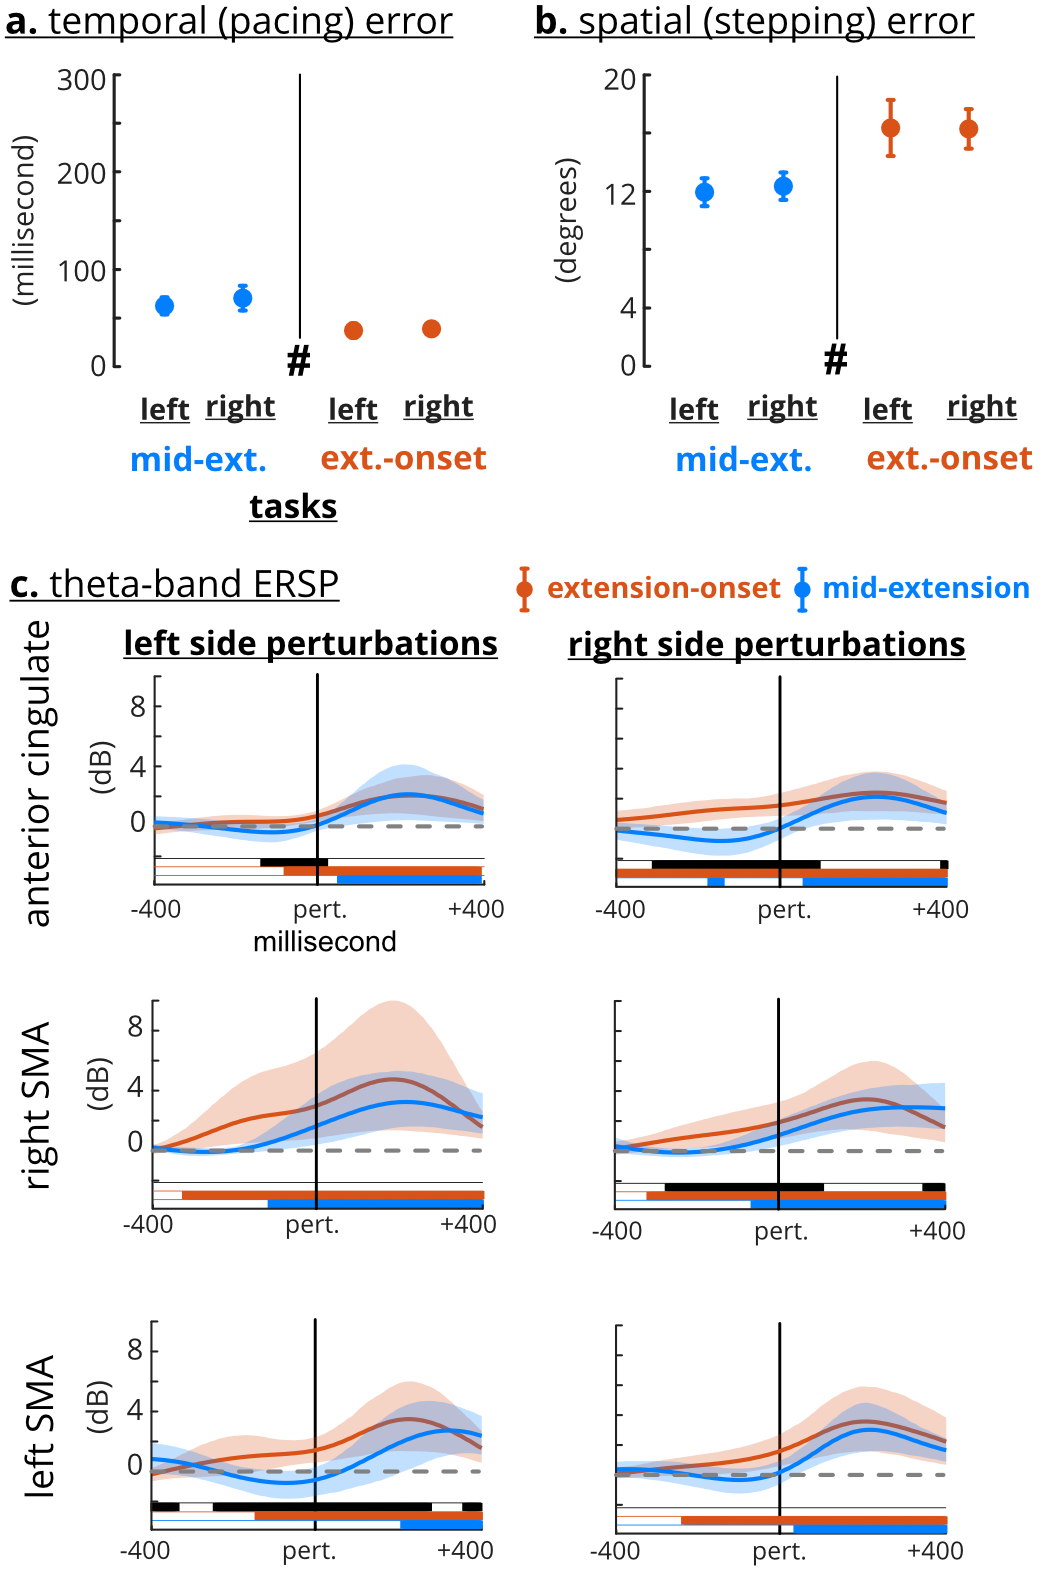
\includegraphics{../img/hyp3 - perturb timing-fdr.jpg}}
\caption{\textbf{Motor errors and theta-band ERSP across perturbation timings.} \textbf{a.} and \textbf{b.} Task type (mid-extension vs. extension-onset) was a significant factor for motor errors. Error bars indicate confidence interval (CI). \textbf{c.} Extension-onset perturbations had greater anterior cingulate and ipsilateral theta-band ERSP before the perturbation event (the solid vertical line). The theta-band ERSP was not significantly different after the perturbation event, except for the left SMA ipsilateral task. Shaded area indicates confidence interval. Black bars indicate significant difference between perturbation timing. Colored bars indicate CI clearing zero.}
\label{fig:fig7}
\end{figure}

\subsection{Perturbations at extension-onset had greater theta-band ERSP in motor cortices than at mid-extension}
Group analyses including all perturbed strides revealed differential motor error and cortical responses based on perturbation timing (Figure \ref{fig:fig7}). Comparing motor errors across all perturbed strides revealed that perturbation timing, and not the task side, was a significant factor (rANOVA, temporal timing: F\tsu{(1,16)}=30.5, p<0.0005, temporal side: F\tsu{(1,16)}=2.24, p=0.15, spatial timing: F\tsu{(1,16)}= 27.5, p<0.0005, spatial side: F\tsu{(1,16)}=0.25, p=0.62) (Figure \ref{fig:fig7}a-b). For each side, temporal error was significantly greater during mid-extension than extension-onset and the spatial error was smaller during mid-extension than extension onset (post-hoc paired t-test, temporal right: p<0.0005, temporal left: p=0.001, spatial right: p<0.0005, spatial left: p=0.001). The extension-onset perturbations elicited a significant increase in theta-band ERSP before the perturbation event across the anterior cingulate {and ipsilateral} SMA (Figure \ref{fig:fig7}c). The increased theta-band ERSP for mid-extension perturbations was delayed, occurring after the perturbation event in the anterior cingulate and left SMA but was about -100 ms before the perturbation event in the right SMA. {Only the ipsilateral left SMA showed greater extension-onset theta-band ERSP than mid-extension for more than 100 ms after the perturbation onset.}

\subsection{Cortical lateralization and specialization}
The left and right SMAs demonstrated both contralateral and task-specific lateralization with respect to lower limb extension (Figure \ref{fig:fig8}). The recovery-step desynchronization during the perturbed strides was most prominent in the right SMA for extension-onset tasks and in the left SMA for the mid-extension tasks, indicating presence of task-specific lateralization (Figure \ref{fig:fig8}a, red rectangles). Mid-extension tasks also involved theta desynchronization before the perturbation event in both left and right SMAs (Figure \ref{fig:fig8}a, red dashed rectangles). Similar recovery-step desynchronization was present in the catch strides but were limited to the ipsilateral SMA of the recovery-step leg during extension-onset tasks and to the right SMA for mid-extension tasks (Figure \ref{fig:fig8}b, black and red rectangles). Strong theta synchronization only occurred in the right SMA for mid-extension catch strides just before the end of the catch step (Figure \ref{fig:fig8}b, red dashed rectangles).

\begin{figure}[!h]
    \centerline{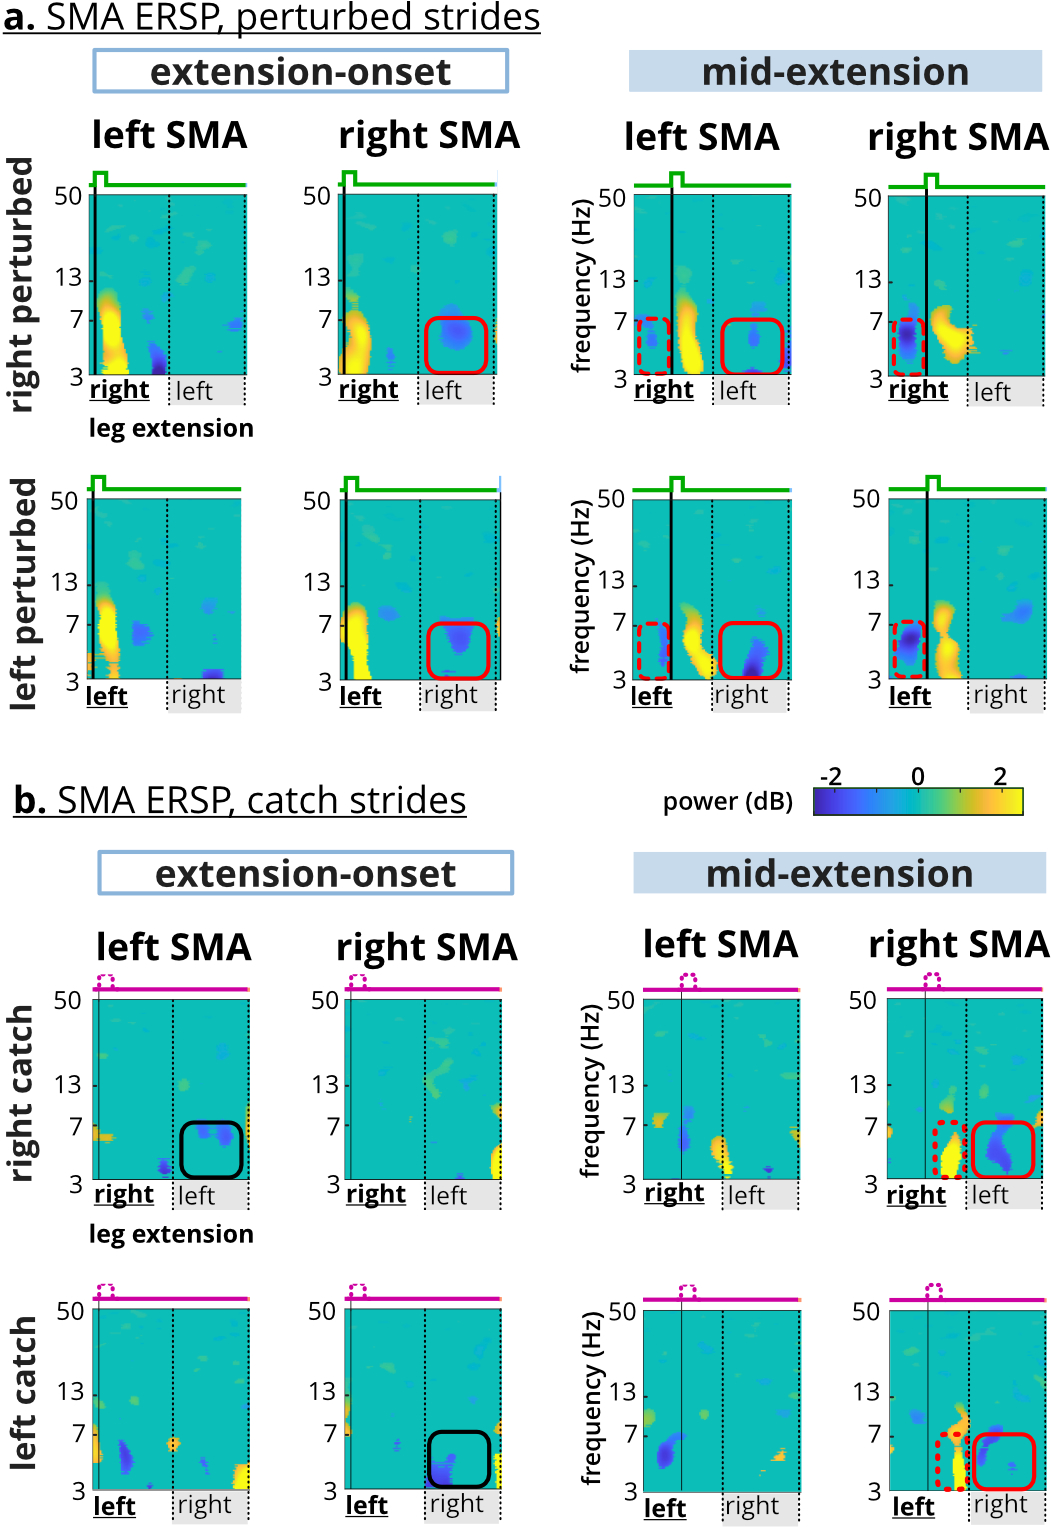
\includegraphics{../img/hyp4- lateraliztion.jpg}}
    \caption{\textbf{Supplementary motor area (SMA) Lateralization.} \textbf{a.} Theta desynchronization in the perturbed recovery step occurred in the right SMA for extension-onset and in the left SMA for the mid-extension (red squares). Only mid-extension perturbations elicited theta desynchronization before the perturbation event (red dashed rectangles). \textbf{b.} Mid-extension catch steps elicited theta synchronization before the end of limb extension (red dashed rectangles). Recovery-step theta desynchronization occurred contralaterally during extension-onset, but only occurred in the right SMA during the mid-extension. Red and black indicate specialized and contralateral lateralization respectively.}
    \label{fig:fig8}
    \end{figure}

\section{Discussion}
\label{sec:Discussion}

We quantified motor and electrocortical responses to frequent mechanical perturbations during recumbent stepping to gain insight on the electrocortical dynamics of locomotor adaptation. We did not observe typical motor error adaptation. Temporal errors {were consistently} \td50ms of the desired pace during perturbed strides and returned to pre-perturbation levels in the post block. Spatial errors did not adapt (decrease) with more exposure to the perturbations and did not return to pre-perturbation levels in the post block. The lack of error-based adaptation behavior coupled with small temporal errors and sustained spatial errors in the post block are indicative of use-dependent learning \cite{Diedrichsen2010-as}. Electrocortical sources in the anterior cingulate cortex and supplementary motor areas showed that perturbations elicited theta synchronization, as expected. {Despite the lack of motor error adaptation, anterior cingulate theta synchronization showed a decreasing trend during late perturbed strides in the right-side tasks.} Interestingly, theta-band ERSP during extension-onset tasks started before the perturbation event, resulting in greater theta synchronization in the anterior cingulate and SMAs preceding the perturbation event compared to mid-extension tasks. Motor cortex lateralization was mostly task-specific, where theta desynchronization occurred during the recovery-step in the right SMA for extension-onset tasks but in the left SMA for the mid-extension tasks. These results highlight that electrocortical and motor responses are not necessarily coupled and that perturbation features such as timing could be tuned to elicit greater involvement of specific brain areas.

The perturbed recumbent stepping protocol did not produce the typical error reduction and rapid wash-out associated with motor adaptation, but instead, revealed sustained errors during the post-perturbation block (Figure \ref{fig:fig4}), suggesting use-dependent learning occurred. {In preliminary analyses, we compared multiple definitions of early and late to determine the robustness of the lack of error-based adaptation in our study. Statistical tests consistently showed no significant difference between early and late, except when early was defined as just the first stride.} When perturbations do not directly hinder achieving the task goal, use-dependent learning emerges more than error-based adaptation \cite{Diedrichsen2010-as}. With use-dependent learning, motor behaviors are modified in the direction of perturbation and sustained longer after removing the perturbations. Here, {we did not provide subjects with any visual feedback of their errors or task performance, so,} matching the stepping pace with the  pacing cues was the more explicit task goal. Because subjects matched the pacing cues well with temporal errors of \td50 ms, which might be imperceptible for active control adjustments \cite{Carpenter1999-lb}, the perturbations did not hinder achieving the task goal. For the less explicit goal of stepping smoothly, however, spatial errors were sustained during perturbed strides and did not wash out during the 2-minute post-perturbation block. During split-crank cycling and split-belt walking where changing muscle recruitment was not an explicit task goal, modified muscular activation patterns were sustained \cite{Alibiglou2011-sc,Maclellan2014-vk}. More recently, a perturbed walking study using brief treadmill belt accelerations during push-off also reported use-dependent learning and sustained post-perturbation gait modifications \cite{Farrens2020-fb}. Longer-lasting locomotor modifications are desirable for gait rehabilitation and warrant further development of use-dependent learning paradigms.

Perturbations during our seated locomotor task elicited significant anterior cingulate theta synchronization that also decreased with time (i.e. adapted) for right-side perturbations, providing new insights about the anterior cingulate role in error monitoring and motor learning. Previous studies have attributed anterior theta synchronization, or the analogous negative deflection in event-related potentials, to physical loss of balance or presence of a postural threat \cite{Adkin2008-fw,Peterson2018-ht}. Our results demonstrated that even without a potential loss of balance, mechanical perturbations during a seated locomotor task can elicit anterior cingulate activity. We also observed {a trend of }adaptation of anterior cingulate theta synchronization for the right-side tasks, which contrasts previous studies that did not observe changes in the anterior cingulate cortex with adaptation but acknowledged a lack of spatial resolution \cite{Haefeli2011-ym,Mierau2015-fd}. Our approach likely had sufficient resolution \cite{Shirazi2019-im, Shirazi2019-ke}, {but we observed a trend of} anterior cingulate adaptation only in the right-side tasks. {Despite consistent motor errors during catch strides, only early catch strides elicited theta synchronization, suggesting that the anterior cingulate perceived early catches as errors, which emphasizes that mechanical perturbations are crucial for anterior cingulate elicitation.} Overall, the sustained anterior cingulate theta power across all tasks during perturbed stepping further supports that the anterior cingulate cortex has a role in error-monitoring. However, {the theta-band adaptation trend} during right-side perturbed stepping suggests that the anterior cingulate also has a role in locomotor learning.


Perturbation timing significantly influenced anterior cingulate theta-band power fluctuations (Figure \ref{fig:fig6}), suggesting that tuning perturbation features can modify and stimulate anterior cingulate activity. The theta-band average ERSP for extension-onset perturbations was greater than mid-extension perturbations. This difference may result from an additional intrinsic anterior cingulate theta synchronization that occurs during limb transitions in unperturbed gait, pedaling, and stepping \cite{Gramann2011-yj,Bulea2015-dv,Kline2016-ci,Enders2016-id}. However, our results did not show significant anterior cingulate activity during pre and post-perturbations strides, partly because our analyses and ICA focused on identifying sources involved in perturbed stepping. The sustained anterior cingulate theta-band elicitation over the entire six minutes of left mid-extension perturbations demonstrates that specific perturbations could be tuned to enhance or extend cortical engagement.

We identified two close but distinct SMA clusters that exhibited specialized lateralization with both theta synchronization and desynchronization. We were able to identify distinct clusters in close proximity using our novel EEG noise rejection process that performs algorithmic parameter sweeping to estimate the most brain sources and an optimal k-means clustering algorithm to identify optimal cortical clusters (Figure \ref{fig:fig3}). The left and right SMAs had clear differences in theta fluctuations (Figure \ref{fig:fig8}), supporting that these SMA clusters were distinct and had specialized responses to the perturbations or motor errors. Theta synchronization occurred exclusively in the right SMA during mid-extension catch steps that had the largest temporal errors (\td250 ms), suggesting that despite the lack of a physical perturbation, the right motor area theta synchronization was still sensitive to a motor error. The right motor and premotor cortices have been linked with monitoring temporal aspects of motor tasks \cite{Mutha2014-ea,Wagner2016-nx}.

Interestingly, theta desynchronization occurred during the recovery step (i.e., the step following a perturbed step) in the right SMA during extension-onset perturbations and in the left SMA during mid-extension perturbations (Figure \ref{fig:fig8}). Previous unperturbed gait studies showed significant theta desynchronization in sensorimotor cortices during mid-stance, but the significance of theta desynchronization specifically is not discussed \cite{Gramann2011-yj,Bulea2015-dv,Enders2016-id,Kline2016-ci}. A recent study demonstrated that theta synchronization and desynchronization corresponds to negative and positive deflections in event-related potentials (ERP) of motor cortex, respectively \cite{Nakagome2020-iv}. As such, ERP studies provide additional possible interpretations for observed theta synchronization and desynchronization in locomotor tasks. For example, a recent study on upper-limb visuomotor perturbations suggested that the presence (or absence) of negative and positive potentials during perturbations indicated different motor learning strategies \cite{Palidis2019-kg}, which aligns with our results.

Limitations of this study include attributing cortical and motor responses to lower-limb extension and {focusing on EEG group-level analyses}. We attributed the perturbations to the action of extending the lower-limb, i.e., left mid-extension perturbation means the perturbation occurred in the middle of extending the left-leg. Our stepping torque analysis (not reported here) and a previous study showed that during arms and legs recumbent stepping, subjects mainly relied on lower-limb extension for higher power demands \cite{Skinner2014-cl}. {Ensemble averaging across strides and subjects is necessary for EEG group-level analysis to reveal event-locked cortical fluctuations} \cite{Makeig1993-jx,Pfurtscheller1999-oi}. {Previous studies had >60 strides per subject for ensemble averaging, inherently increasing their statistical power} \cite{Peterson2018-ht,Wagner2016-nx}. {We had \td10 catch strides and \td50 perturbed strides per subject and yet were still able to observe distinct event-locked spectral fluctuations. Further single trial analysis may provide more insights into the inter-stride cortical variability} \cite{Wagner2019-at,Mierau2015-fd}.

Mechanical perturbations are a robust way to elicit error-related cortical fluctuations and could be tuned to further enhance desired cortical activity. During a seated locomotor task, mechanical perturbations elicited anterior cingulate cortex activity, which decreased with more experience with the right-side perturbations. This supports that the anterior cingulate both monitors errors and learns from them \cite{Holroyd2002-fl}. The left and right SMA clusters demonstrated task-specific lateralization, suggesting that tuning perturbation features such as timing can elicit more desired cortical activity. The uncoupled anterior cingulate activity with motor errors and the specialized SMA fluctuations implicate that cortical feedback may be crucial for closed-loop rehabilitation because motor changes may not adequately reflect cortical dynamics.


% \addbibresource{{\subfix{../refs.bib}}}
\bibliographystyle{ieeetr}
\bibliography{../refs}
% \printbibliography
\end{document}